\chapter{Crittografia Asimmetrica}

Una funzione botola è una funzione facile da computare in una direzione, ma difficile da computare in direzione
opposta. RSA è un esempio di implementazione di funzione di questo tipo.

\section{RSA}

È un algoritmo di crittografia asimmetrico utilizzabile per criptare, decriptare, effettuare autenticazione tramite firma
digitale e scambiare chiavi da usare in seguito per sistemi a cifratura simmetrica.

\noindent È basato sull’elevata complessità computazionale della fattorizzazione in numeri primi, che ne garantisce la sicurezza.

\subsubsection{Generazione delle chiavi}

La generazione delle chiavi per ciascun utente segue i seguenti passi:
\begin{enumerate}
    \item scelti due primi $p$ e $q$ casuali da almeno 2048 bit 
    \item viene calcolato $n=pq$ e $\phi(n)=(p-1)(q-1)$
    \item viene scelto un esponente pubblico $e$ che sia coprimo con $\phi(n)$ (e minore di $n$)
    \item viene calcolato l'esponente privato $d$ tale che il prodotto con l'esponente pubblico 
    sia congruo a 1 modulo $\phi(n)$

    $\rightarrow ed \equiv 1$ $mod$ $\phi(n)$ 
\end{enumerate}

\begin{itemize}
    \item chiave pubblica $k_u = (e,n)$
    \item chiave privata $k_p = (d, p, q)$
\end{itemize} 

\noindent Per la generazione dei parametri:
\begin{itemize}
    \item per trovare $p$ e $q$ vengono generati dei numeri dispari casuali, e poi viene fatto un test di primalità 
    \item per trovare l'esponente privato si utilizza l'algoritmo di Euclide esteso
\end{itemize}

\subsubsection{Cifratura e decifratura}

\begin{itemize}
    \item \textbf{Cifratura:} $c = m^e$ $mod$ $n$
    \item \textbf{Decifratura:} $m = c^d$ $mod$ $n$
\end{itemize}

\subsubsection{Calcolo dell'esponente}

L'operazione di calcola della potenza modulare $x^y$ $mod$ $z$ può essere implementata 
in diversi modi:
\begin{itemize}
    \item \textit{naive:} si moltiplica $x$ per sé stesso per $y$ volte facendo il modulo ad ogni passo, per 
    evitare cifre grandi; poco efficiente siccome la complessità è asintotica a $y$
    \item \textit{left to right:} siano $y_0y_1 \dots y_n$ i bit che formano $y$
    \begin{itemize}
        \item definiamo $y=y_0+2(y_1+2(y_2 \dots +2(y_{n-1}+2y_n)))$
        \item da cui $\Rightarrow x^y = x^{y_0} + 2(x^{y_1}+2(x^{y_2} \dots +2(x^{y_{n-1}} + 2 \cdot x^{y_n})))$
    \end{itemize}
    \item \textit{right to left:} siano $y_0y_1 \dots y_n$ i bit che formano $y$
    \begin{itemize}
        \item definiamo $y = y_0 \cdot 2^0 + y_1 \cdot 2^1 + \dots + y_n \cdot 2^n$
        \item da cui $\Rightarrow x^y = x^{y_0 \cdot 2^0} + x^{y_1 \cdot 2^1} + \dots + x^{y_n \cdot 2^n}$
    \end{itemize}
    
\end{itemize}

\noindent Con gli ultimi due metodi la complessità passa da essere esponenziale a lineare rispetto 
al numero dei bit di $y$.

\newpage
\section{Crittosistema di El-Gamal}

\subsection{Concetto di logaritmo discreto}

\begin{itemize}
    \item Definiamo un gruppo finito $G$ con operazione $\oplus$
    \item Definiamo $H$ il sottogruppo generato da $a$, ovvero $a^i$ con $i < 0$
    \item Definiamo $a \in G$ e $b \in H$
    \item L'unico intero $x$ tale che $a^x = a \oplus a \oplus \dots \oplus a = b$ viene chiamato 
    logaritmo discreto di $b$ in base $a$
\end{itemize}

\noindent Possiamo definire anche come $a^x = b$ $mod$ $N$

$\Rightarrow$ se $N$ è primo, diventa difficile invertire il calcolo

\subsection{Generatori}

\begin{itemize}
    \item definiamo $Z_p=\{0, \dots , p-1\}$
    \item definiamo $Z_p^*$ i numeri di $Z_p$ che sono coprimi con $p$
    \item $g$ è un generatore di $Z_p^*$ se elevandolo a tutte gli elementi di $Z_p$
    si ottengono tutti gli elementi che compongono $Z_p$ stesso
\end{itemize}

\begin{figure}[H]
    \centering
    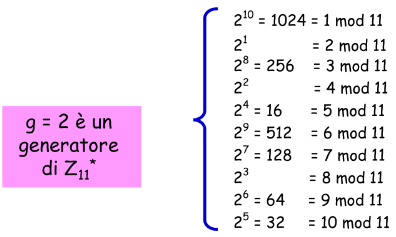
\includegraphics[width=0.6\linewidth]{chapters/chap04/images/generatore.png}
\end{figure}

\subsection{Generazione delle chiavi}

Il crittosistema di El-Gamal si base sul concetto di logaritmo discreto; il processo per 
la generazione delle chiavi è il seguente:
\begin{itemize}
    \item ogni utente genera un numero primo $p$ molto grande e calcola:
    \begin{itemize}
        \item un generatore $g$ di $Z_p^*$
        \item un $\alpha$ casuale compreso tra 1 e $p-1$
    \end{itemize}
    \item la chiave pubblica è $(p, g, \beta)$, con $\beta = g^\alpha$ $mod$ $p$
    \item la chiave privata è $\alpha$
\end{itemize}

\subsection{Cifratura}

\begin{itemize}
    \item codificare il messaggio come un intero $m$ in $Z_p$
    \item scegliere un intero $k$ compreso tra 1 e $p-1$
    \item calcolare $y_1 = g^k$ $mod$ $p$
    \item calcolare $y_2 = m\beta$ $mod$ $p$
\end{itemize}

$\Rightarrow$ il messaggio cifrato corrisponde alla coppia $(y_1, y_2)$

\subsection{Decifratura}
\begin{itemize}
    \item calcolare $z=y_1^\alpha$ $mod$ $p$
    \item calcolare $m = z^{-1} \cdot y_2$ $mod$ $p$, con $z^{-1}$ inverso modulare di $z$
\end{itemize}

